\clearpage
\subsection{Reading a near miss and a false positive from their band edges}
The band-edge thresholds and the gap window test different aspects of a prediction. Figure~\ref{fig:bands} uses the contest's edge convention, plotting larger reported edge values lower on the page. Each horizontal solid level is a CBM or VBM value; its height can be compared across all three columns. The dotted levels show the two contest cutoffs. For a successful candidate, the CBM should lie above its line in the drawing and the VBM below its own line.

\begin{figure}[ht]
\centering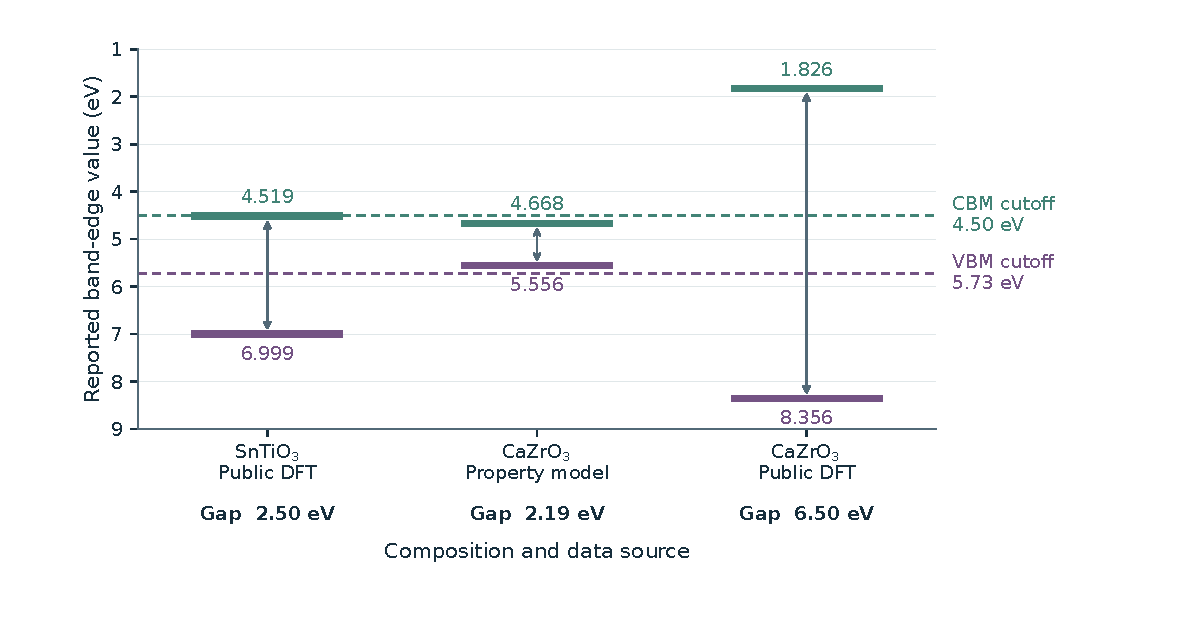
\includegraphics[width=\linewidth]{figures/band_edges.pdf}
\caption{Band-edge levels in eV for the public Q3 winner and the Q3 failure of the seed-26 property model. Arrows span the two edge estimates. Below each column is the separately reported or predicted GLLB-SC gap field used in the objective. Energies follow the file's reference convention.}\label{fig:bands}
\end{figure}

For $\mathrm{SnTiO_3}$, the CBM lies 0.018833 eV beyond its cutoff, a difference too small to resolve easily at the figure scale. For $\mathrm{CaZrO_3}$ the observed edges both pass, but the observed gap is 6.50 eV. It exceeds the upper limit by 3.40 eV and produces the entire observed violation of 46.24.

The middle column explains how the four-property model can rank that material first. It predicts $g=2.1883$ eV, with both small band-edge violations and a passing formation energy, for a total predicted $V=0.2342$. Its independently fitted edges imply $5.5559-4.6680=0.8879$ eV, far from its own gap estimate. In the public DFT record the analogous difference is 6.53 eV, close to the tabulated 6.50 eV. The discrepancy between the model's two estimates of the gap provides a composition-level warning that could be checked before spending a single assay. The following sensitivity test evaluates this warning across all Q3 validation pairs.

\clearpage
\subsection{Can a consistency check rescue a one-choice screen?}
The $\mathrm{CaZrO_3}$ failure suggests a testable diagnostic. Define
\[
 D(z)=\big|\hat g(z)-(\hat v(z)-\hat c(z))\big|.
\]
All three terms are predictions from the property-first model, so the diagnostic could be computed before measuring a candidate. It checks whether the two representations of the gap agree. A small residual can also occur when both representations are wrong in the same direction.

\begin{figure}[ht]
\centering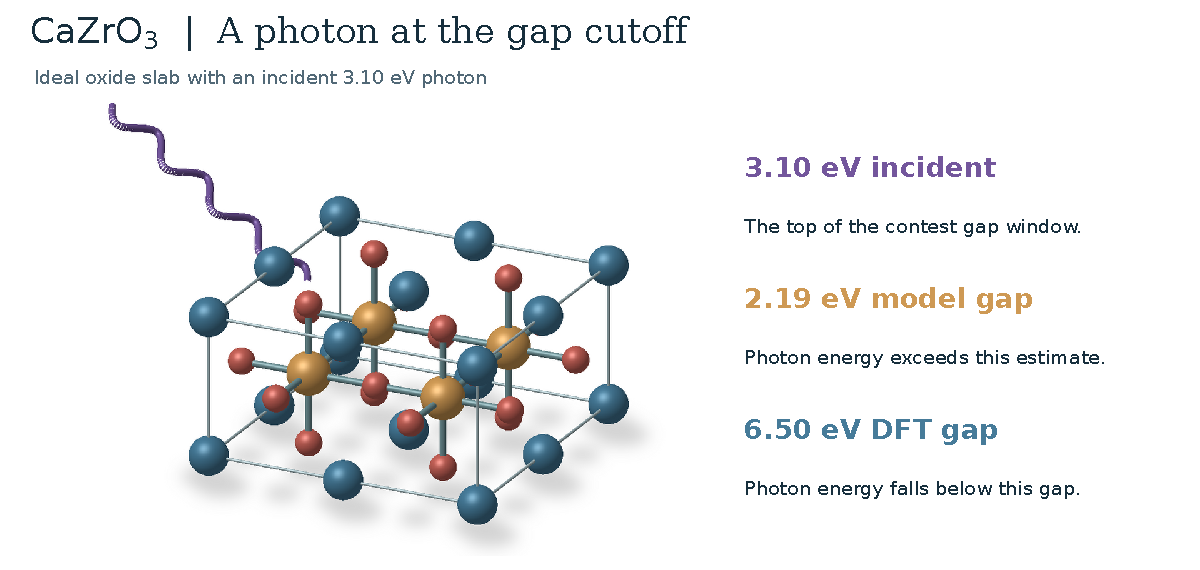
\includegraphics[width=.95\linewidth]{figures/property_tests.pdf}
\caption{An incident photon at the 3.10 eV screening cutoff approaches an ideal fragment of $\mathrm{CaZrO_3}$. The wave is symbolic. Its energy exceeds the model gap but falls below the public DFT gap. This compares energy thresholds only; the files supply no absorption spectrum for this illustration.}\label{fig:physicaltests}
\end{figure}

At 3.10 eV, a photon carries about the energy of 400 nm light ($\lambda=hc/E$). Figure~\ref{fig:physicaltests} uses it to expose the practical consequence of the gap discrepancy. Whether a transition actually absorbs light also depends on selection rules and the optical response.

We test a veto on the 1,701 Q3 validation records: discard predictions with $D>\tau$ and select the remaining candidate with the smallest property-first violation. Table~\ref{tab:veto} reports both seeds, with 26 first in each entry. The same 11 near-targets are available to each fit. Thresholds are exploratory, and this test does not alter the frozen mixture.
\begin{table}[ht]
\caption{Cost of vetoing inconsistent property predictions. Eligible and retained counts refer to distinct Q3 validation records.}\label{tab:veto}
\centering\small\begin{tabular}{lrrr}
\toprule Tolerance (eV) & Eligible records & Near-targets retained & First observed $V$\\\midrule
No veto & 1701 / 1701 & 11 / 11 & 46.24 / 46.24\\
1.00 & 1698 / 1699 & 11 / 10 & 11.25 / 46.24\\
0.50 & 1690 / 1681 & 10 / 9 & 11.97 / 11.25\\
0.25 & 1634 / 1623 & 7 / 5 & 11.97 / 10.88\\
0.05 & 753 / 805 & 0 / 3 & 10.88 / 10.93\\\bottomrule
\end{tabular}
\end{table}

At $\tau=0.50$ the large error on $\mathrm{CaZrO_3}$ is removed for both seeds, yet neither replacement is a near-target. At $\tau=0.05$ the seed-26 screen eliminates every available near-target. Agreement between model outputs can flag a case for inspection. Using that agreement as an automatic rejection criterion sacrifices some of the materials the screen is meant to find.


